\section{Evaluation}

To verify the effectiveness and performance of the domain-level scheduler,
different simulated environments were created. This section presents an
evaluation of the system using QEMU system emulation, focusing on the kernel's
ability to maintain constant time domain scheduling while still showing that
functionality of the within-domain priority scheduler is unaffected. 

\subsection{The blinky example}
\begin{figure}
  \begin{center}
    \include{figures/blinky_timeline}
  \end{center}
  \caption{Timeline of the Blinky Domain Scheduling}\label{fig:blinky_timeline}
\end{figure}

The RISC-V mpu port includes a standard \texttt{mpu\_blinky.c} example. The
example program creates two tasks, a sender and a receiver. The sender adds a
message to a \texttt{Queue} at a set interval, and the receiver reads from the
\texttt{Queue} whenever there is a message available. After a set amount of
message passing, the sender reads from a restricted memory address causing a
pmp fault that gets handled by a custom exception handler. For cross-domain
communication, a similar approach can be used to check that the tasks are still
capable of passing messages to each other. The domain-level scheduler is set up
such that the main function is called with elevated privilege and it is
capable of creating queues and new tasks. The tasks creation is modified to
make use of the new api, such that it creates two new tasks, each in a separate
domain. The scheduling timeline of this modified example is provided in
Figure~\ref{fig:blinky_timeline}.

That is, when the initial program is started and execution is within domain 0,
then domain 0 has given up 2 time slices for the Sender (domain 2), and 2 time
slices for the Receiver domain (Domain 1). As it itself finishes execution, the
rest of its time slices will simply be used by the idle task. Each task is
capable of reading the current domain tick, and the demo simply prints this,
when execution starts. Running the demo produces the following snippet of
output:
\begin{lstlisting}[language={c}]
Sending to task, DomainTick: 4
Message received from task, DomainTick: 2
Sending to task, DomainTick: 4
Message received from task, DomainTick: 2
Sending to task, DomainTick: 4
Message received from task, DomainTick: 2
Sending to task, DomainTick: 4
Message received from task, DomainTick: 2
Sending to task, DomainTick: 4
prvQueueSendTask: trying to access privileged data

=== PMP ACCESS FAULT ===
mcause  = 0x00000005
mepc    = 0x80003730
mtval   = 0x80180001
mstatus = 0x00000080
type    = load
task    = Tx
system halted.
\end{lstlisting}

The output does show some interesting properties with regards to the domain
scheduler. First, although the receive task is scheduled before the sender
task, given that there is no message to read in the Queue, it simply sleeps for
its very first execution, scheduling the idle task. Next, one can see that the
sending happens always at the specified DomainTick 4, and that the receiving
also happens within the expected domain tick 2. Another interesting note is,
that in the very last iteration before the access fault, the receiver task is
never able to receive the final message, as the sender continues uninterrupted
before causing the fault.

\subsubsection{Constant time}
While the previous example shows that the Domain Tick seems constant for
both\footnote{If it varies then the likely culprit is the priority based
scheduler within each domain.}, it does not show that each domain runs for a
constant amount of time before interruptions. To truly show that this runs in
constant time, the evaluation is limited by the tools available. QEMU does not
provide cycle-accurate emulation, and by default makes use of the host system
clock for interrupts, meaning that the demo's execution is dependent on the
rest of the host system. This issue is something that will be discussed later
in Section~\ref{sec:qemu_cycle_accuracy}. QEMU does however provide a flag
known as \texttt{-icount}, which provides deterministic execution from the
guest point of view. Instead of making use of the host interrupt, QEMU instead
makes use of instruction counting to determine elapsed time
\cite{TCGInstructionCounting}. While this by no means is cycle-accurate and
does not take into account any microarchitectural state, it can be used to
approximate the time each domain is allowed to run before a scheduling occurs.

In RISC-V the \texttt{rdcycle} instruction reads XLEN bits of the
\texttt{cycle} counter, which holds a count of the number of clock cycles
executed by the processor core on which the hart is running from an arbitrary
start time in the past. Given FreeRTOS runs with XLEN 32-bit, it is necessary
to also make use of the \texttt{rdcycleh} instruction, to read the upper 32
bits of the cycle counter, to get the true cycle count. This means that one
can find a round trip time of the domain switch in the following fashion:
\begin{lstlisting}[language={c}]
static uint64_t ullPrevMtime = 0;

uint64_t ullMtime;
uint64_t ullMtimeHigh;

asm volatile ("rdtime %0" : "=r"(ullMtime));
asm volatile ("rdtimeh %0" : "=r"(ullMtimeHigh));
ullMtime = ((ullMtimeHigh << 32) | ullMtime);
\end{lstlisting}

By saving the previous cycle count from when this point was last reached and
calculating the round trip time, the demo can be made to print this round trip
time for each domain, producing output like the following:

\begin{verbatim}
...
Sending to task, DomainTick: 4
Round Trip: domain=2 delta=50000
Round Trip: domain=0 delta=50000
Message received from task, DomainTick: 2
Round Trip: domain=1 delta=50000
Round Trip: domain=2 delta=50000
Round Trip: domain=0 delta=50001
Round Trip: domain=1 delta=49999
Round Trip: domain=2 delta=50000
Round Trip: domain=0 delta=50000
Round Trip: domain=1 delta=50000
Round Trip: domain=2 delta=50000
Round Trip: domain=0 delta=50000
Round Trip: domain=1 delta=50000
Round Trip: domain=2 delta=50000
Round Trip: domain=0 delta=50000
Round Trip: domain=1 delta=50000
Sending to task, DomainTick: 4
Round Trip: domain=2 delta=50000
Round Trip: domain=0 delta=50000
Message received from task, DomainTick: 2
...
\end{verbatim}

Which shows that each domain runs in the same number of cycles
with a variance of 1. This variance seems negligible, and could most likely be
attributed in some small discrepancy in how QEMU handles the machine timer
interrupt.

\subsection{Larger Demo}
\begin{figure}
  \begin{center}
    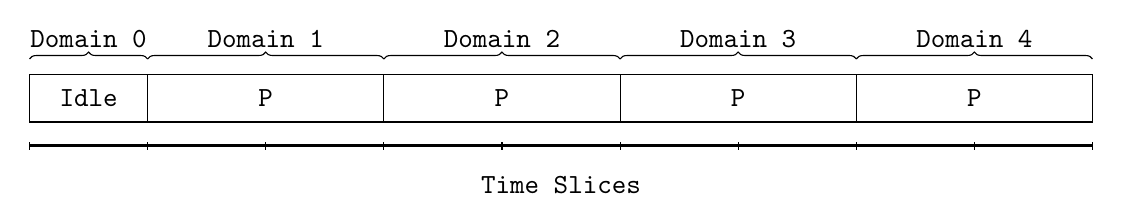
\begin{tikzpicture}[font=\ttfamily]

    % Style for general text nodes
    \tikzset{lbl/.style={inner sep=1pt, align=center}}

    % Define vertical coordinates for rows and labels
    \def\barheight{0.6} % Height of each bar
    \def\vtopprio{1.5}   % Vertical center of the top bar row
    \def\ytimeline{\vtopprio - \barheight} % Vertical position of the minor frames timeline

    % Define standard tick positions
    \def\timeslice{1.5}

    % Domain 0
    \def\tstart{0}
    \def\tend{\timeslice*1}
    \path[draw, decorate, decoration=brace] (\tstart, \vtopprio + 0.5) -- (\tend, \vtopprio + 0.5) node[lbl, midway, above, yshift=0.3em]{Domain 0};
    \draw (\tstart, \vtopprio-\barheight/2) rectangle (\tend, \vtopprio+\barheight/2) 
      node[lbl, midway]{Idle};

    % Domain 1
    \def\tstart{\timeslice*1}
    \def\tend{\timeslice*3}
    \path[draw, decorate, decoration=brace] (\tstart, \vtopprio + 0.5) -- (\tend, \vtopprio + 0.5) node[lbl, midway, above, yshift=0.3em]{Domain 1};
    \draw (\tstart, \vtopprio-\barheight/2) rectangle (\tend, \vtopprio+\barheight/2) 
      node[lbl, midway]{P};

    % Domain 2
    \def\tstart{\timeslice*3}
    \def\tend{\timeslice*5}
    \path[draw, decorate, decoration=brace] (\tstart, \vtopprio + 0.5) -- (\tend, \vtopprio + 0.5) node[lbl, midway, above, yshift=0.3em]{Domain 2};
    \draw (\tstart, \vtopprio-\barheight/2) rectangle (\tend, \vtopprio+\barheight/2) 
      node[lbl, midway]{P};

    % Domain 3
    \def\tstart{\timeslice*5}
    \def\tend{\timeslice*7}
    \path[draw, decorate, decoration=brace] (\tstart, \vtopprio + 0.5) -- (\tend, \vtopprio + 0.5) node[lbl, midway, above, yshift=0.3em]{Domain 3};
    \draw (\tstart, \vtopprio-\barheight/2) rectangle (\tend, \vtopprio+\barheight/2) 
      node[lbl, midway]{P};

    % Domain 4
    \def\tstart{\timeslice*7}
    \def\tend{\timeslice*9}
    \path[draw, decorate, decoration=brace] (\tstart, \vtopprio + 0.5) -- (\tend, \vtopprio + 0.5) node[lbl, midway, above, yshift=0.3em]{Domain 4};
    \draw (\tstart, \vtopprio-\barheight/2) rectangle (\tend, \vtopprio+\barheight/2) 
      node[lbl, midway]{P};

    % Main timeline axis
    \draw[thick] (0, \ytimeline) -- (9*\timeslice, \ytimeline);

    % Intermediate ticks (not all but to give structure)
    \foreach \x in {0, ..., 9} {
         \draw (\x*\timeslice, \ytimeline-0.05) -- (\x*\timeslice, \ytimeline+0.05);
    }

    % Central label below the timeline
    \node[lbl] at ( { 4.5 * \timeslice }, \ytimeline-0.5 ) {Time Slices};

\end{tikzpicture}

  \end{center}
  \caption{Initial domain full setup. P denotes that it is created with a
  single privileged task within.}\label{fig:domain_full}
\end{figure}

A more complex example was also developed to show the capability of creating
tasks within each newly generated domain. The initial setup of the demo can be
seen in Figure~\ref{fig:domain_full}. That is, domain 0 creates 4 new domains
each with a single privileged task. Once domain 0 has created these
tasks, it starts the scheduler and idles. Each domain runs the same privileged task, which can be seen below:
\begin{lstlisting}[language=c]
static void domainPrivileged(void* pvParameters) {
    uint32_t dom_num = (uint32_t) pvParameters;
    TickType_t domain_tick = xTaskGetDomainTick();
    printf ( "Privileged task: %d, DomainTick: %d\n", dom_num, domain_tick);
    static StackType_t xPrivilegedUnStack[ NUM_DOMAINS ][ configMINIMAL_STACK_SIZE ] __attribute__((aligned( configMINIMAL_STACK_SIZE * sizeof(StackType_t) )));

    TaskParameters_t xDomainTaskParameters =
    {
        .pvTaskCode     = domainUnPrivileged,
        .pcName         = "Rx",
        .usStackDepth   = configMINIMAL_STACK_SIZE,
        .pvParameters   = (void* ) dom_num,
        .uxPriority     = mainUNPRIVILEDGE_PRIORITY,
        .puxStackBuffer = xPrivilegedUnStack[dom_num],
        .xRegions       =
        {
            { &_text, _erodata - _text, portMPU_REGION_READ | portMPU_REGION_EXECUTE },
            { &_data, _ebss - _data, portMPU_REGION_READ | portMPU_REGION_WRITE },
            /* NS16550 */
            { (void *)0x10000000UL, 0x1000, portMPU_REGION_READ | portMPU_REGION_WRITE },
            { 0, 0, 0 },
            { 0, 0, 0 },
            { 0, 0, 0 },
            { 0, 0, 0 },
            /* *MUST* reserve one entry for stack */
            { 0, 0, 0 },
        }
        #if ( configENABLE_DOMAINS == 1 )
        ,.pxDomainParameters  = NULL,
        #endif
    };

    TaskHandle_t xDomTask;

    BaseType_t ret = pdFAIL;
    while (ret != pdPASS) {
        ret = xTaskCreateRestricted( &( xDomainTaskParameters ), &xDomTask );
    }

    // This is never reached, Privileged has lower priority than UnPrivileged
    for( ; ; )
    {
    }
}
\end{lstlisting}

Each of the privileged tasks start by printing their domain number and the
current domain tick. Once that is done, they create a new unprivileged task
with a higher priority than themselves. This then immediately schedules the new
task, and the privileged task is never scheduled again. The unprivileged task
that is created is defined as follows:

\begin{lstlisting}[language=c]
static void domainUnPrivileged(void* pvParameters) {
    uint32_t dom_num = (uint32_t) pvParameters;
    TickType_t domain_tick = xTaskGetDomainTick();
    printf ( "UnPrivileged task: %d, DomainTick: %d\n", dom_num, domain_tick);

    TickType_t prev_tick = xTaskGetTickCount();
    TickType_t cur_tick = xTaskGetTickCount();

    for( ; ; )
    {
        cur_tick = xTaskGetTickCount();
        TickType_t domain_tick = xTaskGetDomainTick();
        if (prev_tick != cur_tick) {
            printf ( "Domain %d, Domain Tick %d\n", dom_num, domain_tick);
            prev_tick = cur_tick;
        }
    }
}
\end{lstlisting}
This unprivileged task again starts by printing its domain and the domain tick,
before going into an infinite loop. Within this infinite loop, it checks if a
new tick occurred, and prints its own domain along with the domain tick. The
overall demo is quite simple, but shows the functionality of creating a new
task within a created domain, and one would expect that the provided domain
ticks are constant for each domain. Running this demo with the '-icount' QEMU
flag gives the following output:

\begin{verbatim}
Privileged task: 1, DomainTick: 1
UnPrivileged task: 1, DomainTick: 1
Domain 1, Domain Tick 2
Privileged task: 2, DomainTick: 3
UnPrivileged task: 2, DomainTick: 3
Domain 2, Domain Tick 4
Privileged task: 3, DomainTick: 5
UnPrivileged task: 3, DomainTick: 5
Domain 3, Domain Tick 6
Privileged task: 4, DomainTick: 7
UnPrivileged task: 4, DomainTick: 7
Domain 4, Domain Tick 8
Domain 1, Domain Tick 1
Domain 1, Domain Tick 2
Domain 2, Domain Tick 3
Domain 2, Domain Tick 4
Domain 3, Domain Tick 5
Domain 3, Domain Tick 6
Domain 4, Domain Tick 7
Domain 4, Domain Tick 8
\end{verbatim}

First, we see that the privileged task from domain 1 runs at the expected
domain tick 1. It then creates the unprivileged task within the same tick, and
because the unprivileged task has a higher priority than the privileged task
the priority based scheduler within domain 1 switches out the privileged task
with the unprivileged task all within the same tick. The unprivileged task
reaches the infinite loop, and prints that the domain tick incremented to two,
before looping until its time slice is up. The same sequence follows for the
other domains, before all the unprivileged tasks are the only ones producing
output, where we can see the two time slices given to each of the domains and
how the scheduler is upholding the number of time slices for each domain.

\subsection{QEMU cycle accuracy}\label{sec:qemu_cycle_accuracy}
As mentioned previously, the QEMU virtual machine does not provide cycle
accurate emulation. The closest provided is the instruction-based time counting
as described in \cite{TCGInstructionCounting}. This means that any timing
channel that arises from the microarchitectural shared state cannot be
emulated or diagnosed on the QEMU platform. What can be empirically evaluated
on the platform is a constant time execution path as shown with the previous
domain-level scheduler. In an attempt to gain more true cycle estimations a
QEMU TCG plugin was developed for emulating the cache behaviour of the program
during execution. QEMU provides a cache modelling plugin example
\cite{CacheModellingTCG}. The developed plugin emulated the L1 and L2 cache
with support for flushing the L1 cache on domain switches. While the plugin
functioned correctly in emulation, QEMU was never designed to produce cycle
accurate emulation. When the plugin attempted to update the machine timer
externally, this happened asynchronously and was affected by the host machine
running QEMU, meaning that even with correct cache emulation, the guest OS
would experience non-deterministic execution. The limitations of this approach
and potential alternatives are discussed in
Section~\ref{sec:cycle_accurate_hw}.

\subsection{Limitations}
FreeRTOS was not created with the MPU version in mind. This means that
development on the MPU version of FreeRTOS is quite a recent endeavour and most
likely still subject to change. One clear issue with the aforementioned domain
level scheduler is the inter-domain scheduler itself. FreeRTOS provides two
different modes for tasks, namely the Privileged Mode and the User mode. When a
task is in user mode, it is unable to create any other tasks, as this changes
kernel memory and disables interrupts for the duration of the call. This poses
an issue when wanting to implement strict boundaries between separate domains.
When creating a new domain, if this is initialized with only a User mode task,
then that domain will see no other tasks as the task itself cannot create new
tasks. 

The more subtle problem is that Privileged Mode takes precedence over the
domain separation. Given two domains 0 and 1, each with a single Privileged
mode task within, then these two tasks can always communicate with each other,
as there are no restrictions on what a Privileged task can access. The domain
separation is thus only for User mode tasks, and by no means does it extend to
the Privileged mode tasks within FreeRTOS. Further, the separation itself
requires that the privileged mode tasks within each domain explicitly run
within the allocated time slices as they can disable interrupts via the
FreeRTOS api. One such example is for task creation. When a Privileged mode
task wishes to create another task, FreeRTOS enters a critical section, which
for the RISC-V version disables all interrupts including the machine hardware
interrupt. If the task does not do this carefully, it could delay the domain
level scheduler, which would create a possible timing channel between this
privileged task and a user level task in another domain. This means that the
only cross-domain timing protection enabled via this implementation is between
two User mode tasks running in separate domains.

\subsection{The FreeRTOS kernel is vast}
One requirement for time protection specified within \cite{ge2019} is that the
OS must be partitioned. This includes all system calls, which must be constant
time in regard to available information within each domain. Given that the
domain scheduler implemented creates a copy of the priority based scheduler for
each domain, it can be assumed that a large portion of these system calls
indirectly become constant time in this aspect. Further, as the User mode tasks
are unable to disable any interrupts this would indicate that the shared front
that remains to be partitioned is anything regarding the domain-level scheduler
itself. Given that these do make use of constant-time operations, and domain creation is
restricted to Privileged mode, then it would seem that this requirement might
be met to some extent. However, to truly show this partitioned OS one would
need a full audit of all system calls available for User mode tasks, and make
sure that they are constant time with respect to the domain available
information. As this is something beyond the scope of this thesis, the
implementation can provide no guarantees that it is truly implementing time
protection.
